\chapter{Stokes problem}
\label{chap-stokes}
%\long\def\COMMENT#1{\par\vbox{\hrule\vskip1pt \hrule width.125in height0ex #1\vskip1pt\hrule}}

%\newcommand{\norm}[1]{ |\!|\!| #1 |\!|\!|}
%\newtheorem{theorem}{Theorem}[section]
%\newtheorem{example}{Example}[section]
%\newtheorem{exercise}{Exercise}[section]
%\newtheorem{exercise}{Exercise}[chapter]
%\newtheorem{remark}{Remark}[section]
%\newtheorem{proof}{Proof}[section]


\section{Introduction}
The Stokes problem describes the flow of a slowly moving viscous incompressible Newtonian
fluid.  Let the fluid domain be denoted $\Omega$. We assume that $\Omega$ is a bounded domain in $\mathbb{R}^n$ with a smooth boundary. Furthermore, let $u : \Omega \rightarrow \mathbb{R}^n$ be
the fluid velocity and $p:\Omega \rightarrow \mathbb{R}$ be the fluid pressure.
The strong form of the Stokes problem can then be written as
\begin{eqnarray}
-\Delta u + \nabla p &=& f, \mbox{ in } \Omega,   \\
\nabla \cdot u &=& 0, \mbox{ in } \Omega, \\
u &=& g, \mbox{ on } \partial \Omega_D, \\
\frac{\partial u}{\partial n} - p n  &=& h, \mbox{ on } \partial \Omega_N.
\end{eqnarray}
Here, $f$ is the body force, $\partial \Omega_D$ is the Dirichlet
boundary, while $\partial \Omega_N$ is the Neumann
boundary. Furthermore, $g$ is the prescribed fluid velocity on the
Dirichlet boundary, and $h$ is the surface force or stress on the
Neumann boundary. These boundary condition leads to a well-posed
problem provided that neither the Dirichlet nor Neumann boundaries are
empty.  In case of only Dirichlet conditions the pressure is only
determined up to a constant, while only Neumann conditions leads to
the velocity only being determined up to a constant.

These equations are simplifications of the Navier--Stokes equations for
very slowly moving flow.  In contrast to elliptic equations, many
discretizations of this problem will lead to instabilities.  These
instabilities are particularly visible as non-physical oscillations in
the pressure. The following example illustrate such oscillations.

\begin{example}{Poiseuille flow} \\
One of the most common examples of flow problems that can be solved
analytically is Poiseuille flow. It describes flow in a straight
channel (or cylinder in 3D).  The analytical solution is $u=(y\,
(1-y), 0)$ and $p = 1-x$.  Since the solution is know, this flow
problem is particularly useful for verifying that the code or
numerical method. We therefore begin by discretizing the problem in
the simplest way possible; that is, linear continuous/Lagrange elements
for both velocity and pressure. The results are shown Figure
\ref{fig:stokes1}. Clearly, the velocity is approximated satisfactory,
but the pressure oscillate widely and is nowhere near the actual
solution.
\begin{figure}
\begin{center}
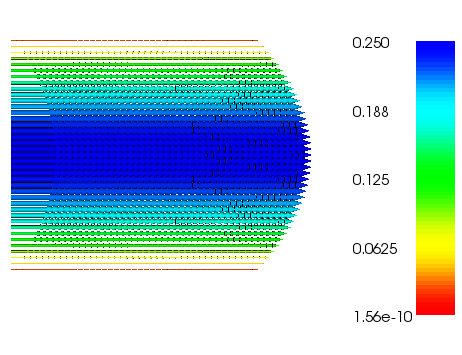
\includegraphics[width=0.45\textwidth]{chapters/Stokes_problem/plots/stokes_velocity.png}
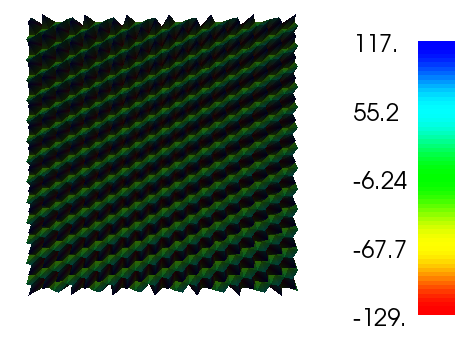
\includegraphics[width=0.45\textwidth]{chapters/Stokes_problem/plots/stokes_pressure_instabilities.png}
\caption{Poiseuille flow solution obtained with linear continuous elements for
both velocity and pressure. The left figure shows the (well-represented) velocity while the right shows
the pressure (with the wild oscillations).}
\label{fig:stokes1}
\end{center}
\end{figure}

% inf56xx-2013/code/stokes/stokes_p1p1.py
\begin{python}
from dolfin import *

def u_boundary(x):
  return x[0] < DOLFIN_EPS or x[1] > 1.0 - DOLFIN_EPS or x[1] < DOLFIN_EPS

def p_boundary(x):
  return  x[0] > 1.0 - DOLFIN_EPS

mesh = UnitSquare(40,40)
V = VectorFunctionSpace(mesh, "Lagrange", 1)
Q = FunctionSpace(mesh, "Lagrange", 1)
#Q = FunctionSpace(mesh, "DG", 0)
W = MixedFunctionSpace([V, Q])

u, p = TrialFunctions(W)
v, q = TestFunctions(W)

f = Constant([0,0])

u_analytical = Expression(["x[1]*(1-x[1])", "0.0"])
p_analytical = Expression("-2+2*x[0]")

bc_u = DirichletBC(W.sub(0), u_analytical, u_boundary)
bc = [bc_u]

a = inner(grad(u), grad(v))*dx + div(u)*q*dx + div(v)*p*dx
L = inner(f, v)*dx

UP = Function(W)
A, b = assemble_system(a, L, bc)
solve(A, UP.vector(), b, "lu")

U, P = UP.split()

plot(U, title="Numerical velocity")
plot(P, title="Numerical pressure")

U_analytical = project(u_analytical, V)
P_analytical = project(p_analytical, Q)

plot(U_analytical, title="Analytical velocity")
plot(P_analytical, title="Analytical pressure")

interactive()
\end{python}



However, when using the second order continuous elements for the velocity and
first order continuous elements for the pressure, we obtain the perfect solution
shown in Figure \ref{fig:stokes2}.
\begin{figure}
\begin{center}
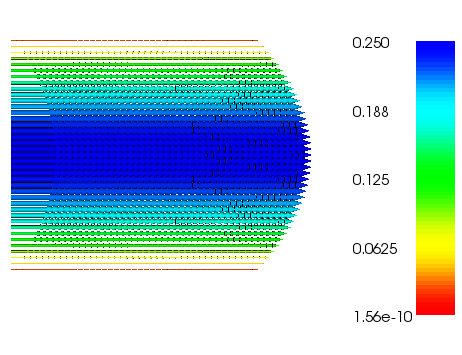
\includegraphics[width=0.45\textwidth]{chapters/Stokes_problem/plots/stokes_velocity.png}
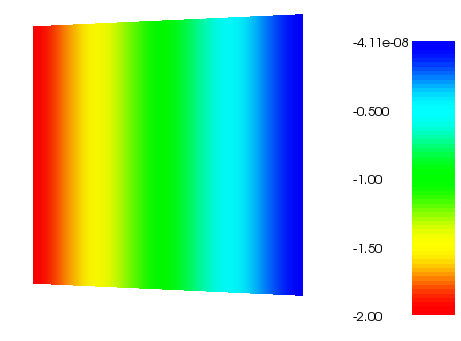
\includegraphics[width=0.45\textwidth]{chapters/Stokes_problem/plots/stokes_pressure.png}
\caption{Poiseuille flow solution obtained with quadratic continuous elements for the
velocity and linear continuous elements for the pressure. The left figure shows the velocity while the right shows
the pressure. Both the velocity and the pressure are correct.}
\label{fig:stokes2}
\end{center}
\end{figure}
\end{example}

The previous example demonstrates that discretizations of the Stokes problem may lead
to, in particular, strange instabilities in the pressure. In this chapter we will describe why this
happens and several strategies to circumvent this behaviour.

\section{Finite Element formulation}

Let us first start with a weak formulation of Stokes problem:
Find $u\in H^1_{D,g}$ and $p\in L^2$.
\begin{eqnarray*}
a(u,v) + b(p,v) &=& f(v), \quad v\in H_{D,0}^1\\
b(q,u) &=& 0,\quad q\in L^2,
\end{eqnarray*}
where
\begin{eqnarray*}
a(u,v) &=& \int\nabla u : \nabla v \dx, \\
b(p,v) &=& \int p \, \nabla \cdot v \dx, \\
f(v) &=& \int f\, v \dx + \int_{\Omega_N} h \, v \, \ds  .
\end{eqnarray*}
Here
$H^1_{D,g}$ contains functions  in $H^1$ with trace $g$ on $\partial \Omega_D$.
To obtain symmetry we have substituted $\hat{p} = - p$ for the pressure
and is referint to $\hat{p}$ as p.

As before the standard finite element formulation follows directly from the weak formulation:
Find $u_h\in V_{g,h}$ and $p_h\in Q_h$ such that
\begin{eqnarray}
\label{eq:stdGalerkin1}
a(u_h, v_h ) + b(p_h, v_h) &=& f(v_h),\quad \forall v_h\in V_{0,h}, \\
\label{eq:stdGalerkin2}
b(q_h, u_h) &=& 0,\quad \forall q_h \in Q_h .
\end{eqnarray}
Letting $u_h=\sum_{i=1}^n u_i N_i$, $p_h=\sum_{i=1}^m p_i L_i$, $v_h=N_j$, and $q_h=L_j$
we obtain a linear system on the form
\begin{equation}
\left[ %matrix
	\begin{array}{cc}
	A & B^T\\
	B & 0
	\end{array}
\right]
\left[ %vector
	\begin{array}{c}
	u\\
	p
	\end{array}
\right]
=
\left[ %vector
	\begin{array}{c}
	f\\
	0
	\end{array}
\right]
\label{la:stokes}
\end{equation}
Here
\begin{eqnarray}
A_{ij} = a(N_i,N_j) &=& \int\nabla N_i \nabla N_j \dx, \\
B_{ij} = b(L_i,N_j) &=& \int\nabla L_i \, N_j \dx.
\end{eqnarray}
Hence, $A$ is $n\times n$, while $B$ is $m\times n$,
where $n$ is the number of degrees of freedom for the velocity field, while
$m$ is the number of degrees of freedom for the pressure.



Is the system \eqref{la:stokes} invertible?  For the moment, we assume that the submatrix $A$ is invertible. This is typically the case for
Stokes problem. We may then perform blockwise Gauss elimination:
That is,
we multiply the first equation with $A^{-1}$ to obtain
\[u = A^{-1}f - A^{-1}B^Tp\]
Then, we then insert $u$ in the second equation to get
\[0 = Bu = BA^{-1}f - BA^{-1}B^Tp\]
i.e we have removed $v$ and obtained an equation only involving $p$:
\[BA^{-1}B^Tp = BA^{-1}f\]
This equation is often called the pressure Schur complement. The question is then reduced to whether $BA^{-1}B^T$ is invertible.
Consider the follwing two situations:

\begin{tabular}[h]{lcr}
\setlength{\unitlength}{0.090in}
\begin{picture}(15,15)
\thinlines
\put(1,0){\line(0,3){3}}
\put(0.7, 0){\line(1,0){0.7}}
\put(0.7, 3){\line(1,0){0.7}}
\put(-1,1.5){$m$}
\thicklines
\put(2,0){\framebox(9,3){$B$}}

\thinlines
\put(1.9,13.6){\line(9,0){9}}
\put(1.9, 13.8){\line(0,-1){0.5}}
\put(11, 13.8){\line(0,-1){0.5}}
\put(5.5,14){$n$}
\thicklines
\put(2,4){\framebox(9,9){$A$}}

\put(12,0){\framebox(3,3){$0$}}
\put(12,4){\framebox(3,9){$B^T$}}
\end{picture}
\vspace{\unitlength}

\qquad   v.s \qquad

\setlength{\unitlength}{0.090in}
\begin{picture}(15,15)
\thinlines
\put(1,0){\line(0,9){9}}
\put(0.7, 0){\line(1,0){0.7}}
\put(0.7, 9){\line(1,0){0.7}}
\put(-1,4.5){$m$}
\thicklines
\put(2,0){\framebox(3,9){$B$}}

\thinlines
\put(1.9,13.6){\line(3,0){3}}
\put(1.9, 13.8){\line(0,-1){0.5}}
\put(5, 13.8){\line(0,-1){0.5}}
\put(2.5,14){$n$}
\thicklines
\put(2,10){\framebox(3,3){$A$}}

\put(6,0){\framebox(9,9){$0$}}
\put(6,10){\framebox(9,3){$B^T$}}
\end{picture}
\vspace{\unitlength}
\end{tabular}

Clearly, the right most figure is not invertible since $n \ll  m$ and
the $0$ in the lower right corner dominates. For the left figure on might expect that the
matrix is non-singular since $n \gg m$, but it will depend on $A$ and $B$. We have already
assumed that $A$ is invertible, and we therefore ignore $A^{-1}$ in $BA^{-1}B^T$.
The question is then whether $BB^T$ is invertible.

\setlength{\unitlength}{0.090in}
\begin{picture}(15,15)
\thicklines
\put(0,6){\framebox(9,3){$B$}}
\put(10,0){\framebox(3,9){$B^T$}}
\put(14,7){$=$}

\thinlines
\put(16,9.6){\line(3,0){3}}
\put(15.9, 9.8){\line(0,-1){0.6}}
\put(19, 9.8){\line(0,-1){0.6}}
\put(15.5,11){\small{$m\!\times\!m$}}
\thicklines
\put(16,6){\framebox(3,3){}}
\label{BBinvertible}
\end{picture}
\vspace{\unitlength}

As illustrated above, $B B^T$ will be a relatively small matrix compared to
$B^T$ and $A$ as long as $n  \gg m$. Therefore, $B B^T$  may therefore be non-singular.
To ensure that $B B^T$ is invertible, it is necessary that
\[\operatorname{kernel}(B^T)=0,\ \textrm{where}\ B \ \textrm{is}\ m\times n\]
An equvialent statement is that
\begin{equation}
\max_v\ (v,B^Tp) > 0\quad \forall p .
\label{max1}
\end{equation}
Alternatively,
\begin{equation}
\max_v\ \frac{(v,B^Tp)}{\|v\| } \ge \beta \|p\| \quad \forall p.
\label{max2}
\end{equation}
which obviously may be written 
\begin{equation}
\max_v\ \frac{(B v,p)}{\|v\| } \ge \beta \|p\| \quad \forall p.
\label{max22}
\end{equation}

Here, $\beta > 0$. We remark that \eqref{max1} and \eqref{max2} are equivalent for a finite dimensional matrix.
However, in the infinite dimentional setting of PDEs \eqref{max1} and \eqref{max2} are different.
Inequality \eqref{max1} allow $(v, B^T p)$ to approach zero, while \eqref{max2} requires a lower bound.
For the Stokes problem, the corresponding condition is crucial:
\begin{equation}
\sup_{v\in H^1_{D,g}}\ \frac{(p, \nabla\cdot u) }{\|u\|_1\ } \ge \beta \|p\|_0 > 0, \quad  \forall p\in L^2
\label{infsup:cont}
\end{equation}

Similarly, to obtain order optimal convergence rates, that is
\[\|u-u_h\|_1 + \|p-p_h\|_0 \le Ch^k\|u\|_{k+1} + Dh^{\ell+1}\|p\|_{\ell+1}\]
where $k$ and $\ell$ are the ploynomial degree of the velocity and the pressure, respectively,
the celebrated \emph{Babuska-Brezzi condition} has to be satisfied:
\begin{equation}
\sup_{v\in V_{h,g}}\ \frac{(p, \nabla\cdot v) }{\|v\|_1\ } \ge \beta \|p\|_0 > 0, \quad  \forall p\in Q_h
\label{infsup:disk}
\end{equation}
We remark that the discrete condition \eqref{infsup:disk} does not follow from \eqref{infsup:cont}.
In fact, it has been a major challenge in numerical analysis
to determine which finite element pairs $V_h$ and $Q_h$ that meet this condition.

\begin{remark}
For saddle point problems on the form \eqref{eq:stdGalerkin1}-\eqref{eq:stdGalerkin2} four conditions
have to be satisfied in order to have a well-posed problem: \\
Boundedness of $a$:
\begin{equation}
\label{remark1}
a(u_h, v_h) \le C_1 \|u_h\|_{V_h} \|v_h\|_{V_h}, \quad \forall u_h, v_h \in V_h,
\end{equation}
and boundedness of $b$:
\begin{equation}
\label{remark2}
b(u_h, q_h) \le C_2 \|u_h\|_{V_h} \|q_h\|_{Q_h},  \quad \forall u_h \in V_h,  q_h \in Q_h,
\end{equation}
Coersivity of $a$:
\begin{equation}
\label{remark3}
a(u_h, u_h) \ge C_3 \|u_h\|^2_{V_h} , \quad \forall u_h \in Z_h,
\end{equation}
where $Z_h=\left\{u_h \in V_h \ | \ b(u_h, q_h) = 0, \  \forall q_h\in Q_h\right\}$ and "coersivity" of $b$:
\begin{equation}
\label{remark4}
\sup_{u_h\in V_h} \frac{b(u_h, q_h)}{\|u_h\|_{V_h}} \ge C_4 \|q_h\|_{Q_h} , \quad \forall q_h \in Q_h.
\end{equation}
For the Stokes problem, \eqref{remark1}-\eqref{remark3} are easily verified, while \eqref{remark4} often
is remarkably difficult unless the elements are designed to meet this condition.
We remark also that condition \eqref{remark3} strictly speaking only needs to be valid on a subspace of $V_h$
but this is not important for the Stokes problem. 
\end{remark}



\section{Examples of elements}
\subsection{The Taylor-Hoood element}
The Taylor-Hood elements are quadratic for the velocity and linear for pressure, i.e., 
the $i$'th basis function of the velocity and pressure are of the form
\begin{eqnarray*}
u:\ N_i &=& a_i + b_i x + c_i y + d_i xy + e_i x^2 + f_i y^2, \\
p:\ L_i &=& k_i + l_i x + m_i y.
\end{eqnarray*}
And the basis functions are continuous across elements.
For the Taylor-Hood element we have the following error estimate:
\[\|u-u_h\|_1 + \|p-p_h\|_0 \le Ch^2 (\|u\|_{3} + \|p\|_{2}).\]
The generalization of the Taylor--Hood element to higher order, that is 
$P_k-P_{k-1}$, satisfies the Brezzi conditions (on reasonable meshes). 
For the Taylor-Hood element of higher order we have the following error estimate:
\[\|u-u_h\|_1 + \|p-p_h\|_0 \le Ch^k (\|u\|_{k+1} + \|p\|_{k}).\]


\subsection{The Crouzeix--Raviart element}
This element is linear in velocity and constant in pressure. Hence, the $i$'th basis functions are of the form:
\begin{eqnarray*}
v:\ N_i &=& a_i + b_i x + c_i y\\
p:\ L_i &=& a_i
\end{eqnarray*}
The $v$ element is continuous \emph{only} in the mid-point of each side, and the $p$ element is discontinuous. The Crouzeix-Raviart element satisifies 
the inf-sup condition, but is non-conforming because it is only continuous at the mid-point of each element. The non-conformity 
does not affect the approximation properties for the Stokes problem, but can not be used if the 
$-\Delta u - \nabla p = f$  
is replaced with the more "physically correct"  
$-\nabla \cdot \epsilon(u) - \nabla p = f$, where $\epsilon=\frac{1}{2}(\nabla + \nabla^T)$ is the symmetric gradient.  
For the Crouzeix--Raviart element we have the following error estimate:
\[\|u-u_h\|_1 + \|p-p_h\|_0 \le Ch (\|u\|_{2} + \|p\|_{1})\]
The element may be generalized to odd, but not even orders. 


\subsection{The P1-P0 element}

The P1-P0 element is perhaps the most natural element to consider as it consists of combining continuous piecewise linear functions for the velocity with piecewise constants
for the pressure. This combination often work quite well, and this puzzled the community for quite some time. However, this combination is not inf-sup stable 
and oscillations in the pressure may occur.


\subsection{The P2-P0 element}

$P_2-P_0$ element is a popular element that  satisfies the Brezzi conditions. 
An advantage with this approach is that mass conservation is
maintained elementwise. However, the approximation properties of the pressure is one order lower than that for the Taylor-Hood element
and consequently the velocity approximation is also formally, in general,  reduced by one order, i.e.,  
\[\|u-u_h\|_1 + \|p-p_h\|_0 \le C_0 h^2\|u\|_{2} + C_1 h\|p\|_{2}\]
The $P_2-P_0$ element can be generalized to higher order. 
In fact,  $P_k-P_{k-2}$, satisfies the Brezzi conditions for $k\ge 2$. Here, the pressure element $P_{k-2}$
may in fact consist of both continuous and discontinuous polynomials. 
The discontinuous polynomials then has the advantage of providing 
mass conservation, albeit at the expence of many degrees of freedom 
compared with the continuous variant. 


\subsection{The Mini element}
The mini element is linear in both velocity and pressure, but with one degree of freedom added per element since it is well-known that elements that are linear in both $v$ and $p$ will not satisfy the inf-sup condition. The extra degree of freedom is in 2D constructed such it is a cubic polynomial which is zero at all element faces. 
For example, on the reference element, the barycentric coordinates $x$, $y$, and $1-x-y$ are all zero at their respective faces. Hence, the composition 
$xy(1-x-y)$ is zero at all element faces. 
The barycentric coordinates can be used for this purpose on any element and also in higher dimensions.   
The function is often called the bubble function as its support is local to one element and is zero at the element faces. 
For the Mini element we have the following error estimate:
\[\|u-u_h\|_1 + \|p-p_h\|_0 \le C_0 h\|u\|_{2} + C_1 h^2\|p\|_{2}\]
We notice that the convergence rate for the velocity is linear, hence the extra bubbles bring stability but does not increase approximation
order. 

\section{Stabilization techniques to circumvent the Babuska-Brezzi condition}
Stabilization techniques typically replace the system:
\begin{eqnarray*}
Au + B^Tp &=& f \\
Bu &=& 0
\end{eqnarray*}
with an alternative system
\begin{eqnarray*}
Au + B^Tp &=& f \\
Bu -\epsilon Dp &=& \epsilon d ,
\end{eqnarray*}
where $\epsilon$ is properly chosen and $D$ is a positive, but not necessarily positive definite,  matrix.

To see that we obtain a nonsingular system we again multiply the first
equation with $A^{-1}$ and then factorize:
\begin{eqnarray*}
u &=& A^{-1}f - A^{-1}B^Tp \\
Bu &=& BA^{-1}f - BA^{-1}B^Tp  = \epsilon d + \epsilon Dp \\
(BA^{-1}B^T + \epsilon D)p &=& BA^{-1}f - \epsilon d
\end{eqnarray*}
If $D$ is nonsingular then
$(BA^{-1}B^T + \epsilon D)$ will be is nonsingular since both $D$ and $BA^{-1}B^T$ are positive (only $D$ is positive definite however).

Factorizing for $p$ we end up with a \emph{Velocity-Schur complement}. Solving for $p$ in the second equation and inserting the expression for $p$ into the first equation we have
\begin{eqnarray*}
p &=& (-\epsilon D)^{-1}(\epsilon d - Bu)\\
&\Downarrow&\\
Au + B^T(-\epsilon D)^{-1}(\epsilon d-Bu) &=& f\\
(A + \frac{1}{\epsilon}B^TD^{-1}B)u &=& f + D^{-1}d
\end{eqnarray*}
$(A + \frac{1}{\epsilon}B^TD^{-1}B)$ is nonsingular since $A$ is nonsingular and $B^TD^{-1}B$ is positive.
%---end section Alternative Stabilization---

At least, three techniques have been proposed for stabilization. These are:
\begin{enumerate}
\item $\nabla\cdot v + \epsilon\Delta p = 0 $. Pressure stabilization. Motivated through mathematical intuition (from the convection-diffusion equation).
\item $\nabla\cdot v  -\epsilon p = 0 $. Penalty method. Typically, one uses the Velocity-Schur complement
\item $\nabla\cdot  -\epsilon\frac{\partial p}{\partial t} = 0 $. 
	Artificial compressibility. A practical method as one adds the
  possibility for time stepping.
\end{enumerate}

\noindent
In other words, these techniques sets $D$ to be
\begin{enumerate}
	\item $D=A$
	\item $D=M$
	\item $D=\frac{1}{\Delta t}M$
\end{enumerate}
where $A$ is the stiffness matrix (discrete laplace operator) and $M$ is the mass matrix.


\section{Exercises}

\begin{exercise}
Show that the conditions \eqref{remark1}-\eqref{remark3} are satisfied for
$V_h = H^1_0$ and $Q_h=L^2$.
\end{exercise}
\begin{exercise}
Show that the conditions \eqref{remark1}-\eqref{remark3} are satisfied for
Taylor--Hood and Mini discretizations.
(Note that Crouzeix--Raviart is non-conforming so it is more difficult to prove these conditions
for this case.)
\end{exercise}
\begin{exercise}
Condition \eqref{remark4} is difficult to prove. However, if we assume that
$V_h = L^2$ and $Q_h=H^1_0$, you should be able to prove it. (Hint: This
is closely related to Poincare's inequality.)
\end{exercise}

\begin{exercise}
Test other finite elements for the Poiseuille flow problem. Consider $P_1-P_0$, $P_2-P_2$, $P_2-P_0$, as
well as the Mini and Crouzeix--Raviart element.
\end{exercise}

\begin{exercise}
Implement stabilization for the Poiseuille flow problem and use first order linear elements
for both velocity and pressure.
\end{exercise}

\begin{exercise}
In the previous problem the solution was a second order polynomial in the velocity and
first order in the pressure. We may therefore obtain the exact solution and it
is therefore difficult to check order of convergence for higher order methods with
this solution. In this exercise you should therefore
implement the problem $u=(sin(\pi y), cos( \pi x)$, $p=sin(2 \pi x)$, and $f = -\Delta u - \nabla p$.
Test whether the approximation is of the expected order for $P_4-P_3$, $P_4-P_2$, $P_3-P_2$, and $P_3-P_1$.

\end{exercise}

\begin{exercise}
Implement the Stokes problem with analytical solution $u=(sin(\pi y), cos( \pi x)$, $p=sin(2 \pi x)$, and $f = -\Delta u - \nabla p$ 
on the unit square.  Consider the case where you have Dirichlet conditions on the sides
'x=0', 'x=1' and 'y=1' while Neumann is used on the last side (this way we avoid the 
singular system associated with either pure Dirichlet or pure Neumann problems).    
Then determine the order of the approximation of wall shear stress on the side 'x=0'. 
The wall shear stress on the side 'x=0' is $\nabla u \cdot t$ where $t=(0,1)$ is the tangent along 'x=0'.
\end{exercise}




%\section{Further reading}


